\begin{center}
\fbox{\fbox{\parbox{6.5in}{\centering
\begin{flushleft}

\vspace{2mm}
\hspace{5mm}
\textbf{\underline{Haripunkti leidmine}}

\vspace{2mm}
\hspace{5mm}
Eelnevalt nägime, et ruutfunktsiooni $y=ax^{2}+bx+c$ graafikuks on parabool ning et sellel paraboolil\\ \hspace{5mm} on ka haripunkt (kõige madalam või kõrgeim punkt).

\vspace{2mm}
\hspace{5mm}
Haripunkt asub punktis

\begin{equation}
\label{37_eq1}
H(x_{h}; y_{h})
\end{equation}

\hspace{5mm}
Koordinaadid $x_{h}$ ja $y_{h}$ saab leida järgmiste valemitega:

\begin{equation}
\label{37_eq2}
\boxed{x_{h}=-\dfrac{b}{2a}}
\end{equation}

\hspace{5mm}
kus $b$ on ruutfunktsiooni $y=ax^{2}+bx+c$ lineaarliikme $bx$ ees olev kordaja ning $a$ on ruutliikme $ax^{2}$\\ \hspace{5mm} ees olev kordaja.

\begin{equation}
\label{37_eq3}
\boxed{y_{h}=ax_{h}^{2}+bx_{h}+c}
\end{equation}

\hspace{5mm}
kus $x_{h}$ on valemist \ref{37_eq2} saadud väärtus ning tegurid $a$, $b$, $c$ esialgse ruutfunktsiooni liikmete kordajad.

\vspace{2mm}
\hspace{5mm}
\textbf{Näiteks:}

\vspace{2mm}
\hspace{5mm}
Leiame funktsiooni $y=3x^{2}-5x+1$ haripunkti. Kasutame valemeid \ref{37_eq1} - \ref{37_eq3}.

\[x_{h}=-\dfrac{b}{2a} \hspace{3mm} \longrightarrow \hspace{3mm} \left[ \begin{tabular}{c}
$y=ax^{2}+bx+c$\\
$y=3x^{2}-5x+1$\\
ehk: $a=3$ ning $b=-5$.
\end{tabular} \right] \hspace{3mm} \longrightarrow \hspace{3mm} x_{h}=-\dfrac{(-5)}{2\cdot 3} = \dfrac{5}{6} \]

\vspace{2mm}
\[ y_{h}=ax_{h}^{2}+bx_{h}+c \hspace{3mm} \longrightarrow \hspace{3mm} \left[ \begin{tabular}{c}
$y=3x^{2}-5x+1$\\
$a=3$, $b=-5$\\
$c=1$, $x_{h}=\dfrac{5}{6}$
\end{tabular} \right]  \hspace{3mm} \longrightarrow \hspace{3mm} y_{h}=3 \cdot \left( \dfrac{5}{6}\right)^{2} -5 \cdot \dfrac{5}{6} +1 = -\dfrac{39}{36} \]

\hspace{5mm}
Järelikult haripunkti koordinaadid on $H\left( \dfrac{5}{6};-\dfrac{39}{36} \right)$ 

\hspace{5mm}
\begin{center}
\begin{minipage}{7cm}
  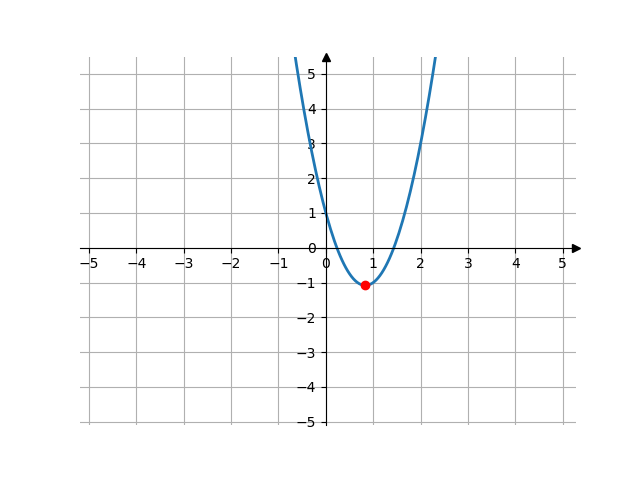
\includegraphics[width=7cm]{37_joonis1.png}
  \captionof{figure}{$y=3x^{2}-5x+1$ haripunkt $H$.}
  \label{37_joonis1}
\end{minipage}
\end{center}

\end{flushleft}
}}}
\end{center}

\pagebreak

\begin{center}
\fbox{\fbox{\parbox{6.5in}{\centering
\begin{flushleft}

\vspace{2mm}
\hspace{5mm}
\textbf{\underline{Ruutvõrrandi valem}}

\vspace{2mm}
\hspace{5mm}
Ruutvõrrandi üldine kuju: 

\begin{equation}
\label{37_eq4}
ax^{2}+bx+c=0
\end{equation}

\vspace{2mm}
\hspace{5mm}
Ruutvõrrandi lahendeid saab leida järgmise üldise valemiga:

\begin{equation}
\label{37_eq5}
\boxed{x_{1,2}=\dfrac{-b \pm \sqrt{b^{2}-4ac}}{2a}}
\end{equation}

\vspace{2mm}
\hspace{5mm}
\textbf{Näiteks:} Lahenda võrrand $3x^{2}-4x=4$

\vspace{2mm}
\hspace{5mm}
Enne valemi \ref{37_eq5} rakendamist, tuleb viia võrrand üldisele kujule nagu \ref{37_eq4} (ehk paneme kogu asja\\ \hspace{5mm} võrduma nulliga).

\[3x^{2}-4x=4 \hspace{3mm} \longrightarrow \hspace{3mm} 3x^{2}-4x-4=0 \]

\hspace{5mm}
Nüüd rakendame valemit \ref{37_eq5}.

\[x=\dfrac{-b \pm \sqrt{b^{2}-4ac}}{2a} = \dfrac{-(-4) \pm \sqrt{(-4)^{2}-4 \cdot 3 \cdot (-4)}}{2 \cdot 3} = \dfrac{4 \pm \sqrt{64}}{6}=\dfrac{4 \pm 8}{6} \]

\hspace{5mm}
Esimese lahendi leiame kui asendame $\pm$ märgi asemele $+$ märgi.

\[ x_{1}=\dfrac{4+8}{6}=\dfrac{12}{6}=2 \]

\hspace{5mm}
Teise lahendi leiame kui asendame $\pm$ märgi asemele $-$ märgi.

\[ x_{2}=\dfrac{4-8}{6}=\dfrac{-4}{6}=-\dfrac{2}{3} \approx -0.667 \]

\vspace{2mm}
\hspace{5mm}
Vastus: Võrrandi lahendid on $x_{1}=2$ ja $x_{2}=-\dfrac{2}{3}$


\vspace{5mm}
\hspace{5mm}
\textbf{\underline{Diskriminant}}

\vspace{2mm}
\hspace{5mm}
Valemis \ref{37_eq5} ruutjuure all olevat osa $b^{2}-4ac$ nimetatakse \textbf{diskriminandiks}. Tähistame seda edaspidi\\ \hspace{5mm} tähega $D$, ehk $D=b^{2}-4ac$.

\vspace{2mm}
\hspace{5mm}
Peatükkis \ref{35_peatükk} mainiti, et ruutjuurt negatiivsest arvust võtta ei saa. Kuidas siis käituda, kui\\ \hspace{5mm} ruutvõrrandi diskriminant (ehk valemis \ref{37_eq5} ruutjuure all olev osa) on negatiivne? Uurime kolme\\ \hspace{5mm} erinevat juhtu, kuidas ruutvõrrandi lahendite arv sõltub diskriminandist:

\vspace{2mm}
\hspace{5mm}
\textbf{1)} $\mathbf{D>0}$

\vspace{2mm}
\hspace{5mm}
Kui diskriminant D on nullist suurem (ehk kui ruutvõrrandi ruutjuure all olev avaldis on positiivse\\ \hspace{5mm} väärtusega), siis on ruutvõrrandil kaks erinevat reaalarvulist lahendit.

\[ x_{1}=\dfrac{-b-\sqrt{D}}{2a} \hspace{5mm} \text{ja} \hspace{5mm} x_{2}=\dfrac{-b+\sqrt{D}}{2a} \]
  
\vspace{2mm}
\hspace{5mm}
\textbf{2)} $\mathbf{D=0}$

\vspace{2mm}
\hspace{5mm}
Kui diskriminant D on võrdne nulliga (ehk kui ruutvõrrandi ruutjuure all olev avaldis on null), siis on\\ \hspace{5mm} ruutvõrrandil kaks võrdset reaalarvulist lahendit.

\[x_{1}=x_{2}=-\dfrac{b}{2a} \]

\end{flushleft}
}}}
\end{center}




\begin{center}
\fbox{\fbox{\parbox{6.5in}{\centering
\begin{flushleft}

\vspace{2mm}
\hspace{5mm}
\textbf{3)} $\mathbf{D<0}$

\vspace{2mm}
\hspace{5mm}
Kui diskriminant D on nullist väiksem ehk negatiivne (teisisõnu, kui ruutvõrrandi ruutjuure all olev\\ \hspace{5mm} avaldis on negatiivne), siis ruutvõrrandil reaalarvulised lahendid \textbf{puuduvad.} 

\vspace{2mm}
\hspace{5mm}
Kui ruutvõrrandil puuduvad reaalarvulised lahendid, ei tähenda see, et võrrandil üldse lahendeid ei ole.\\ \hspace{5mm} Reaalarvude hulka võib laiendada ka nii, et lahend leiduks ka negatiivse diskriminandi korral, kuid see\\ \hspace{5mm} viiks meid juba kompleksarvude domeeni. Sealsed rajad on ekslemise jaoks liiga petlikud ning enne\\ \hspace{5mm} sinna teele asumist tuleks meil oma praegustes sammudes kindlam olla.

\vspace{2mm}
\hspace{5mm}
\textbf{Näited:}

\vspace{2mm}
\hspace{5mm}
1) Leiame võrrandi $2x^{2}-4x+2=0$ lahendid.

\[x=\dfrac{-(-4)\pm \sqrt{(-4)^{2}-4 \cdot 2 \cdot 2 }}{2 \cdot 2} = \dfrac{4 \pm \sqrt{0}}{4}=\dfrac{4\pm 0}{4}=\begin{tabular}{c}
$x_{1}=1$\\
$x_{2}=1$
\end{tabular} \]

\vspace{2mm}
\hspace{5mm}
2) Leiame võrrandi $x^{2}+5x+9=0$ lahendid.

\[ x=\dfrac{-(5) \pm \sqrt{(5)^{2} -4 \cdot 1 \cdot 9} }{2 \cdot 1}= \dfrac{-5 \pm \sqrt{ -11}}{2} = \left[ \begin{tabular}{c}
D<0\\
lahendid puuduvad
\end{tabular}
\right] \]

\vspace{5mm}
\hspace{5mm}
\textbf{\underline{Taandatud ruutvõrrandi valem}}

\vspace{2mm}
\hspace{5mm}
Ruutvõrrand, milles ruutliikme $ax^{2}$ kordaja $a$ on 1, nimetatakse \textbf{taandatud ruutvõrrandiks}. Selle\\ \hspace{5mm} üldine kuju on järgmine: 

\begin{equation}
\label{37_eq6}
x^{2}+px+q=0
\end{equation}

\hspace{5mm}
Taandatud ruutvõrrandi puhul saab kasutada alternatiivset ruutvõrrandi lahendivalemit:

\begin{equation}
\label{37_eq7}
\boxed{x=-\dfrac{p}{2} \pm \sqrt{\left( \dfrac{p}{2}\right)^{2}-q}}
\end{equation}

\hspace{5mm}
Igat ruutvõrrandit võib viia taandatud kujule, jagades kogu võrrandit kordajaga $a$.

\vspace{5mm}
\hspace{5mm}
\textbf{Näiteks:} Viime võrrandi $2x^{2}+3x-2=0$ taandatud kujule.

\[ 2x^{2}+3x-2=0 \hspace{3mm} \bigg| : 2  \]
\[ \dfrac{2x^{2}}{2}+\dfrac{3x}{2} - \dfrac{2}{2}=0 \hspace{3mm} \longrightarrow \hspace{3mm} x^{2}+\dfrac{3}{2}x-1=0\]

\vspace{2mm}
\hspace{5mm}
Leiame lahendid valemiga \ref{37_eq7}.

\[ x=-\dfrac{3}{2 \cdot 2} \pm \sqrt{\left(\dfrac{3}{2 \cdot 2} \right)^{2}-(-1)} = -\dfrac{3}{4} \pm \sqrt{1.5625}= -0.75 \pm 1.25 = \begin{tabular}{c}
$x_{1}=-0.75 + 1.25 = 0.5$\\
$x_{2}=-0.75 - 1.25 = -2$
\end{tabular} \]

\vspace{2mm}
\hspace{5mm}
Vastus: Võrrandi lahendid on $x_{1}=0.5$ ja $x_{2}=-2$.

\vspace{2mm}
\hspace{5mm}
Tegelikult saab igat ruutvõrrandit lahendada üldise ruutvõrrandi lahendivalemiga \ref{37_eq5}, mille tõttu võib\\ \hspace{5mm} taandatud ruutvõrrandi lahendivalem \ref{37_eq7} jääda just kui kasutuks ja üleliigseks. Kuid tegelikult on\\ \hspace{5mm} taandatud ruutvõrrandil \ref{37_eq7} üks suur eelis: \textbf{Viète teoreem}.


\end{flushleft}
}}}
\end{center}


\begin{center}
\fbox{\fbox{\parbox{6.5in}{\centering
\begin{flushleft}

\vspace{5mm}
\hspace{5mm}
\textbf{\underline{Viète'i teoreem*}}

\vspace{2mm}
\hspace{5mm}
Taandatud ruutvõrrandi $x^{2}+px+q=0$ kordajad $p$ ja $q$ avalduvad lahendite kaudu järgmiselt: 


\begin{equation}
\label{viete}
\boxed{
\begin{tabular}{c}
$ x_{1} \cdot x_{2}= q$\\ 
$ x_{1} + x_{2}=-p$
\end{tabular}}
\end{equation}

\hspace{5mm}
Ehk kui on teada ruutvõrrandi lahendid $x_{1}$ ja $x_{2}$, siis võib leida ka taandatud ruutvõrrandi kordajad $p$\\ \hspace{5mm} ja $q$ (ehk saame leida lahendite kaudu esialgse võrrandi). Ning loomulikult saab ka vastupidi leida\\ \hspace{5mm} kordajate kaudu lahendid.

\vspace{2mm}
\hspace{5mm}
Mõned märkused seoses Viete'i teoreemiga:
\begin{itemize}
\item $q$ on negatiivne, kui $x_{1}$ ja $x_{2}$ on erimärgilised, kuid positiivne, kui $x_{1}$ ja $x_{2}$ on samamärgilised.
\item Kui $x_{1}$ ja $x_{2}$ korrutis on positiivne (nad on samamärgilised), siis positiivse summa puhul on $x_{1}$ ja $x_{2}$ mõlemad positiivised ning negatiivse summa puhul on $x_{1}$ ja $x_{2}$ mõlemad negatiivsed. 
\item Kui $x_{1}$ ja $x_{2}$ korrutis on negatiivne (nad on erimärgilised), siis positiivse summa puhul on positiivne $x$ suurem negatiivsest $x$ - st ning negatiivse summa puhul on negatiivne $x$ suurem positiivsest $x$ - st.
\end{itemize}

\end{flushleft}
}}}
\end{center}


\vspace{0.5cm}

\textbf{Märkmed}\\
\vspace{2mm}
\begin{mdframed}[style=graphpaper]
\vspace{12cm}
\end{mdframed}
